\documentclass[russian]{eskdtext}
\usepackage[T2A]{fontenc}
\usepackage[utf8]{inputenc}
\usepackage[russian]{babel}
\DeclareTextSymbol{\No}{T2A}{"9D}
%\ESKDdepartment{Организация}
%\ESKDcompany{Организация1}
%\ESKDclassCode{31 1398}
\ESKDtitle{Автоматизированная система контроля исполнения и доведения документов}
\ESKDdocName{Техническое задание}
\ESKDsignature{АСКИДД 2019.0001}
\ESKDauthor{\scriptsizeФамилия~И.~О}
%Утверждающая надпись
%\ESKDtitleApprovedBy{Должность}{Фамилия~И.~О}
%Согласующая надпись
%\ESKDtitleAgreedBy{Должность}{Фамилия~И.~О}
%Исполнители
%\ESKDtitleDesignedBy{Главный инженер АМО ЗИЛ}{Петров~И.~И}
\ESKDtitleDesignedBy{Должность автора}{Фамилия~И.~О}
\ESKDcolumnI{\smallАвтоматизированная система контроля исполнения и доведения документов. Техническое задание}


%\renewcommand{\ESKDagreedName}{\cyr\CYRS\cyro\cyrg\cyrl\cyra\cyrs\cyro\cyrv\cyra\cyrn\cyro}


\begin{document}
%=================================================================
%=============== ТИТУЛЬНЫЙ ЛИСТ ======================================
%=================================================================
\maketitle

%=================================================================
%=============== СОДЕРЖАНИЕ ======================================
%=================================================================

\tableofcontents
\newpage

%=================================================================
%=============== ТЕКСТОВКА =======================================
%=================================================================
\section{Наименование и шифр, основание, заказчик, сроки выполнения}
\subsection{Наименование работы}
Автоматизированная система контроля исполнения и доведения документов.

Шифр: АСКИДД.

\subsection{Заказчик}
Университет.
\newline
Шифр: АСКИДД

\subsection{Исполнитель}
Учебно-методический отдел.

\subsection{Сроки выполнения}
Январь 2019 г. -- Январь 2020 г.

\section{Цели и задачи выполнения работы}
Целью проведения работы является создание автоматизированной системы обеспечивающей хранение электронных документов (приказов, приказаний, планов и др.), первичный контроль их доведения (в части касающейся) до должностных лиц организации, контроль и учёт докладов об исполнении.
Задачи работы:
\begin{enumerate}
	\item разработать структурно-функциональную схему системы;
	\item сформулировать требования к программному обеспечению, необходимому для разработки и функционирования системы;
	\item сформулировать технически требования для обеспечения функционирования системы;
	\item сформулировать перечень показателей качества функционирования системы;
	\item сформулировать требования к количеству и квалификации сотрудников, обеспечивающих работу системы;
	\item обеспечить государственную регистрацию результата работы;
	\item разработать техническую документацию.	
\end{enumerate}


Проектируемая система обеспечивает:
\begin{itemize}
	\item фиксацию в процессе регистрации всех поставленных на контроль документов и указаний вышестоящих должностных лиц;
	\item проверку доведения документа до исполнителя в срок;
	\item напоминание исполнителям и руководителям подразделений о приближении или истечении сроков исполнения документов;
	\item внесение данных о передаче документа от исполнителя исполнителю или изменении сроков исполнения документов;
	\item информирование вышестоящих должностных лиц о ходе исполнения документов;
	\item внесение в регистрационную форму данных об исполнении документов (снятии документа с контроля);
	\item составление аналитических справок по сроковому контролю за исполнением документов.
\end{itemize}

\section{Технические и функциональные требования}
\subsection{Состав системы}
Автоматизированная система контроля исполнения и доведения документов состоит из следующих компонентов:
\begin{itemize}
	\item модуль организации интерфейса пользователя;
	\item модуль обработки запросов пользователей;
	\item система управления базой данных;
	\item прокси-сервер и static-секция файлового хранилища.
\end{itemize}

В наиболее общем виде архитектура разрабатываемой системы представлена на рис.\ref{fig:arch}
\begin{figure}
	\centering
	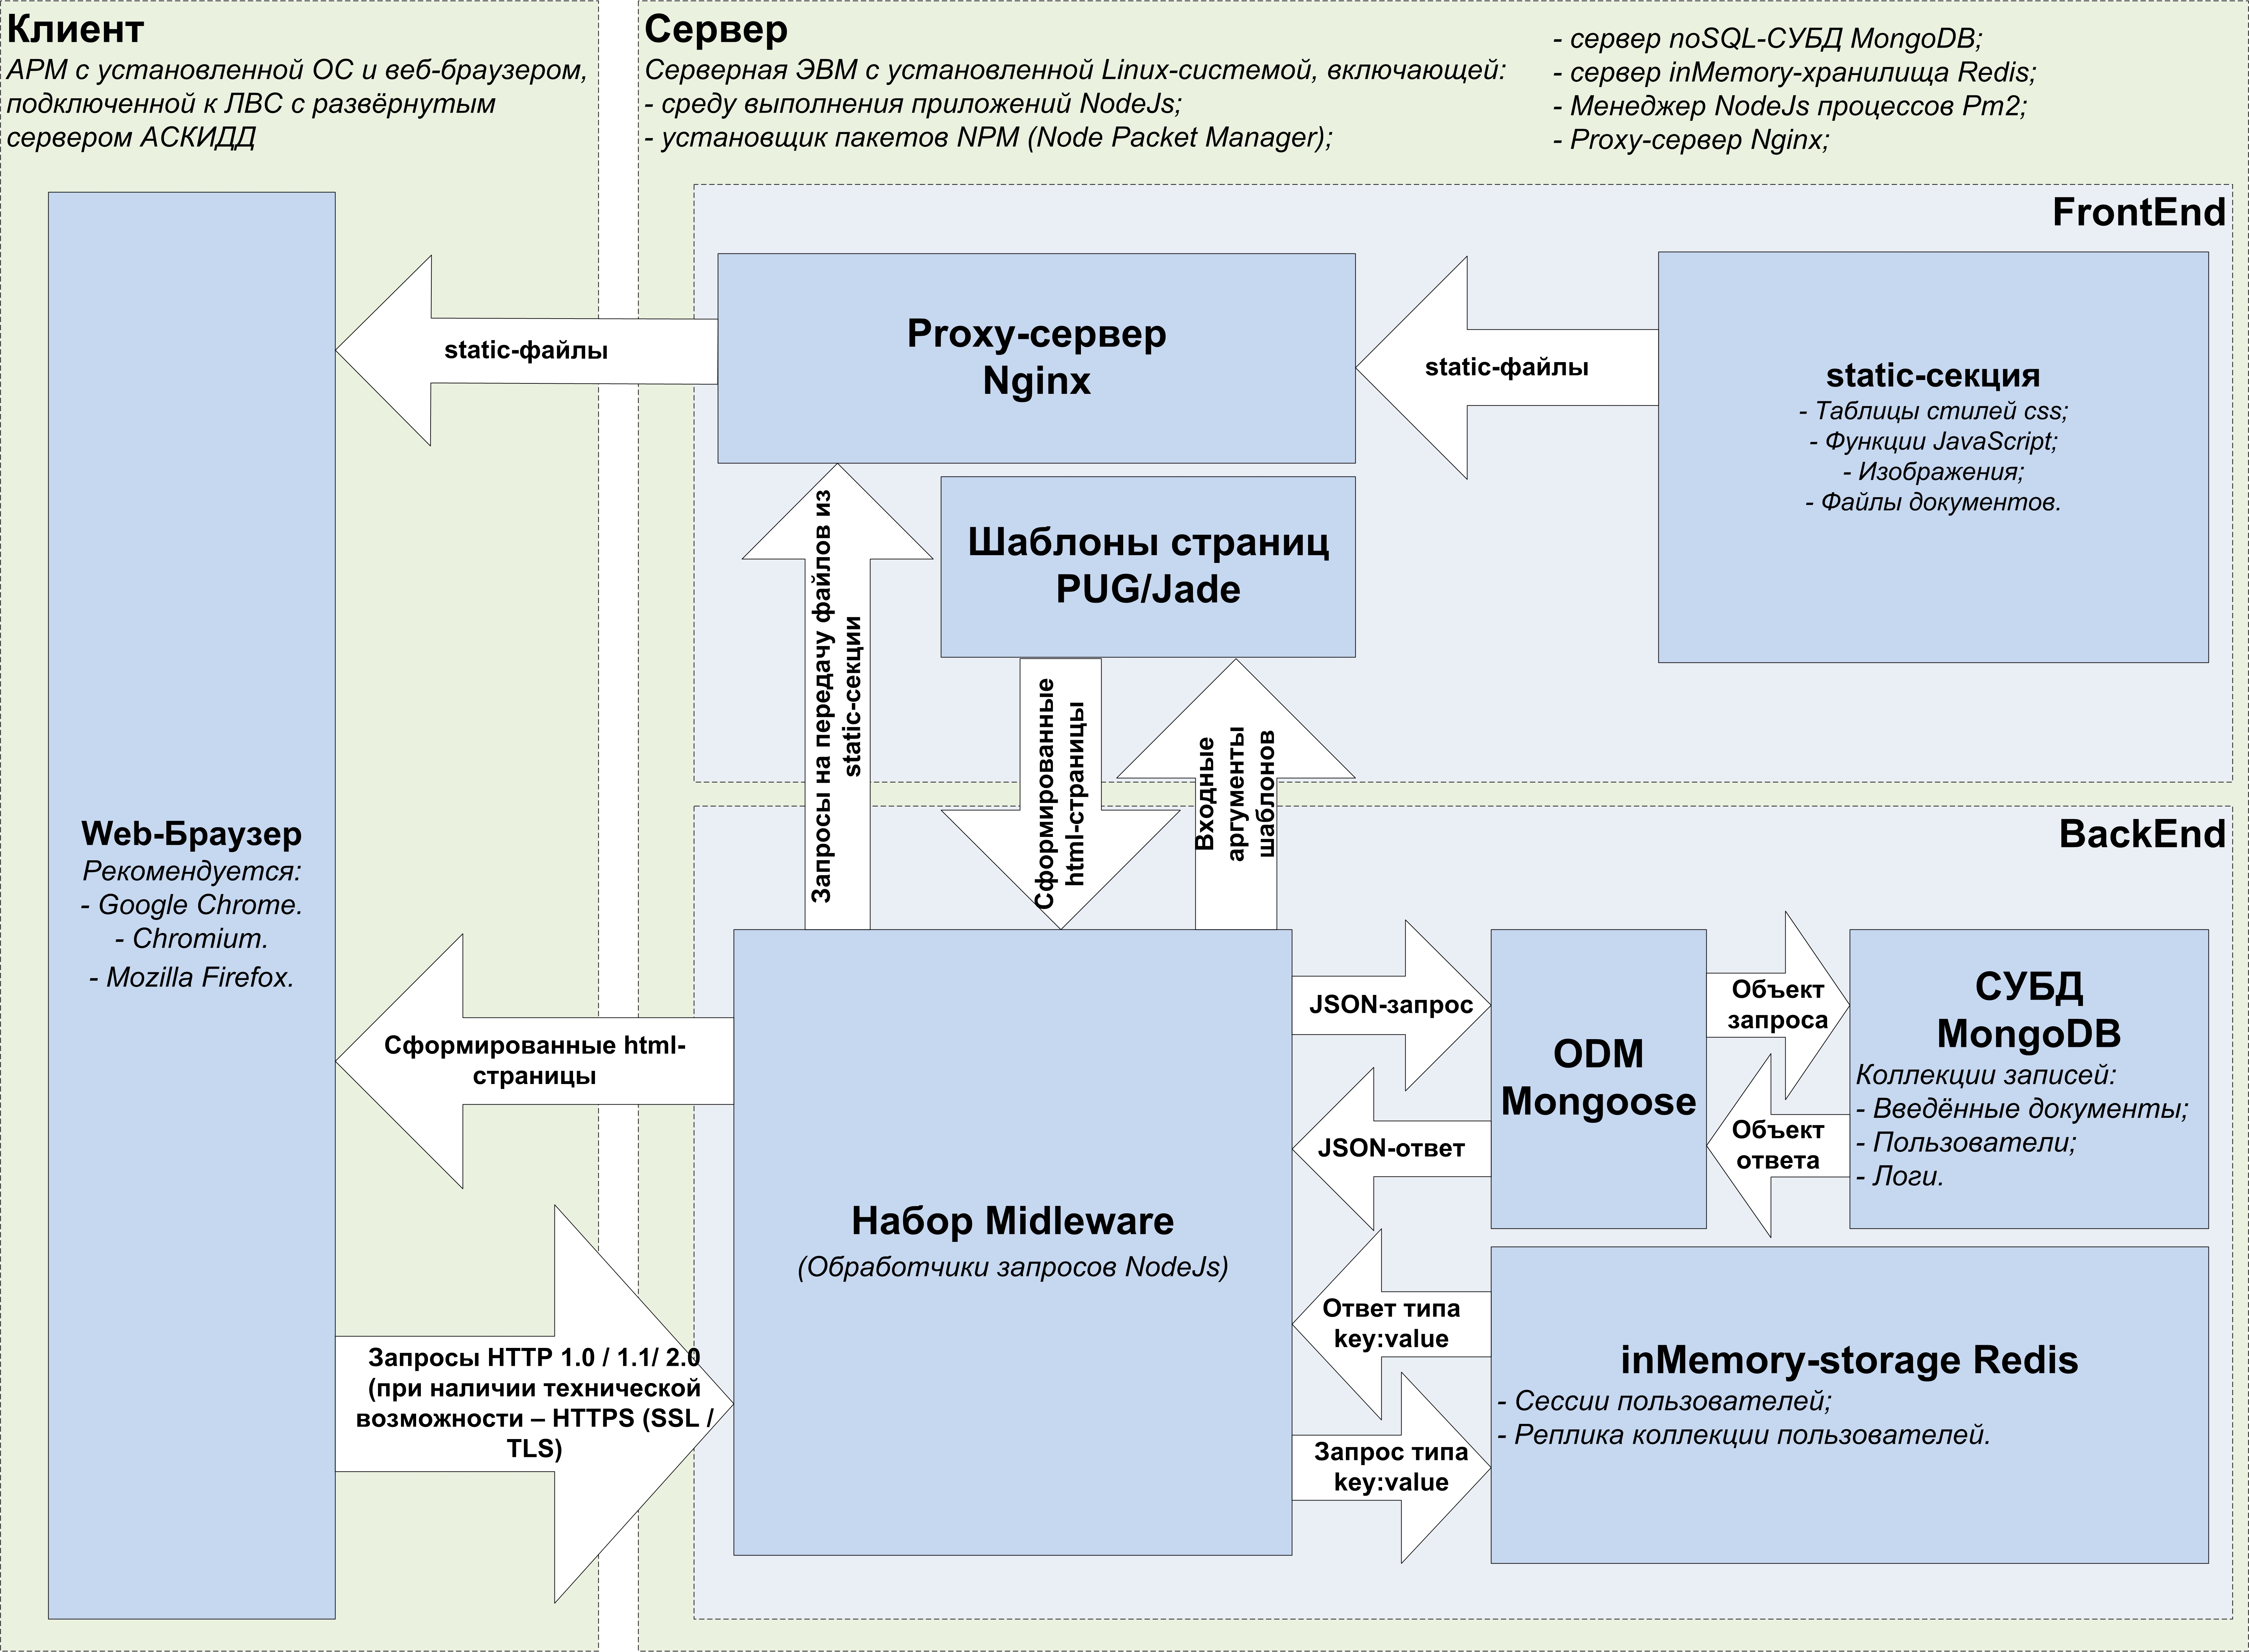
\includegraphics[width=1.0\linewidth]{img/archs_jpeg}
	\caption[Архитектура]{Архитектура основного приложения}
	\label{fig:arch}
\end{figure}

\subsection{Роли пользователей в системе}
Простые пользователи -- сотрудники и должностные лица структурных подразделений, которые непосредственно используют информационные ресурсы системы.

Модераторы -- это простые пользователи системы, которые имеют возможность управления документами в системе (добавлять, редактировать, просматривать и удалять).

Администраторы -- сотрудники имеющие возможность управления учётными записями пользователей, просмотра диагностических сообщений в системе, а также обладающие правами модераторов.

Управление ролями пользователей осуществляется в интерфейсе администратора (админ-панель).

\subsection{Требования к разрабатываемой системе}
В результате проведённого анализа, были определены основные требования к автоматизированной системе контроля исполнения и доведения документов:
\begin{itemize}
	\item Основное приложение разрабатывается в соответствии с концепцией <<веб-клиент>>;
	\item Возможность горизонтального масштабирования системы без изменения общей архитектуры приложения;
	\item Использование свободно-распространяемого программного обеспечения с открытыми исходными кодами;
	\item Минимально-необходимый функционал системы с возможностью наращивания;
	\item Обеспечение необходимого уровня информационной безопасности обработки информации;
	\item Требования к аппаратным средствам, используемым пользователями не предъявляются;
	\item Минимальные требования к аппаратной части серверного оборудования в базовой установке.
\end{itemize}

Основным минимальным требованием, предъявляемом к ЭВМ пользователя является наличие  установленного современного веб-браузера актуальной версии.

Минимальные требования к серверу:
\begin{itemize}
	\item Операционная система Linux Debian 9.6.0 (без графической оболочки);
	\item Объём ОЗУ не менее 512 Мбайт;
	\item Объём НЖМД не менее 10 Гбайт;
	\item Наличие среды выполнения приложений NodeJS;
	\item Наличие СУБД MongoDB;
	\item Наличие СУБД Redis;
	\item Proxy-сервер Nginx;
	\item Менеджер процессов PM2.
\end{itemize}
%%\section{Проба}
%%\cyr\CYRS\cyro\cyrg\cyrl\cyra\cyrs\cyro\cyrv\cyra\cyrn\cyro
%%\cyr\CYRU\cyrt\cyrv\cyre\cyrr\cyrzh\cyrd\cyra\cyryu
%%\cyr\CYRU\cyrt\cyrv\cyre\cyrr\cyrzh\cyrd\cyre\cyrn
%%\cyr\CYRL\cyri\cyrs\cyrt
\end{document}

